\documentclass[a4paper,12pt,twoside]{scrreprt}
% Autor der Vorlage: Klaus Rheinberger, FH Vorarlberg
% 2017-02-20

%% Hilfe: z.B.
% empfohlener Einstieg: http://latex.tugraz.at/  
% https://de.wikibooks.org/wiki/LaTeX-Kompendium:_Schnellkurs:_Erste_Schritte
% https://de.wikibooks.org/wiki/LaTeX-Kompendium:_Schnellkurs
% https://de.wikibooks.org/wiki/LaTeX-Kompendium

%% Pakete:
% Der Befehl \usepackage[latin9]{inputenc} ermöglicht die direkte Angabe von Umlauten. Übrigens lässt sich so auch das Euro-Zeichen direkt eingeben. Auf Betriebssystemen, wie zum Beispiel allen neueren Linux-Distributionen, verwendet man statt \usepackage[latin9]{inputenc} besser \usepackage[utf8]{inputenc}, auf Applesystemen verwendet man \usepackage[macce]{inputenc} (oder das für ältere Modelle gültige \usepackage[applemac]{inputenc}).
\usepackage[utf8]{inputenc}
\usepackage[T1]{fontenc}    % Silbentrennung bei Sonderzeichen
\usepackage{graphicx}       % Bilder einbinden
\usepackage[ngerman]{babel} % Deutsche Sprachanpassungen
\usepackage{csquotes}       % When using babel or polyglossia with biblatex, loading csquotes is recommended to ensure that quoted texts are typeset according to the rules of your main language.
\usepackage{acronym}  % für optionales Abkürzungsverzeichnis
\usepackage{eurosym}  % z. B. \EUR{12345,68}
\usepackage[linktocpage=true]{hyperref} % Links z. B. \href{https://www.wikibooks.org}{Wikibooks home}
\usepackage[bindingoffset=8mm]{geometry}% Bindeverlust von 8mm einbeziehen. Mit dem geometry-Paket können Sie die Ränder auch ganz individuell anpassen.
\usepackage{caption} % Abbildungslegenden
\usepackage{enumitem}
\usepackage{float}
\usepackage{listings}             % Include the listings-package
\usepackage{color}

\definecolor{dkgreen}{rgb}{0,0.6,0}
\definecolor{gray}{rgb}{0.5,0.5,0.5}
\definecolor{mauve}{rgb}{0.58,0,0.82}

\lstset{frame=tb,
  language=Java,
  aboveskip=2mm,
  belowskip=2mm,
  showstringspaces=false,
  columns=flexible,
  basicstyle={\small\ttfamily},
  numbers=none,
  numberstyle=\tiny\color{gray},
  keywordstyle=\color{blue},
  commentstyle=\color{dkgreen},
  stringstyle=\color{mauve},
  breaklines=true,
  breakatwhitespace=true,
  tabsize=3
}

\captionsetup{format=hang, justification=raggedright}

\usepackage[style=alphabetic,citestyle=alphabetic,backend=biber]{biblatex}   % Literaturverweise
%\usepackage[style=numeric,citestyle=numeric,backend=biber]{biblatex}
% biblatex comes with a variety of built-in bibliography/citation style families (numeric, alphabetic, authoryear, authortitle, verbose), and there's a growing number of custom styles:
% https://de.sharelatex.com/learn/Biblatex_citation_styles
% https://de.sharelatex.com/learn/Biblatex_bibliography_styles
\addbibresource{Zotero-Beispiele.bib}    % Zotero-Beispiele.bib ist die verwendete Bibtex-Datei 
% Anstatt die Bibtex-Datei selber zu erstellen, kann sie z. B. aus einer Zotero-Sammlung zu BibTeX exportiert werden.


%% Einstellungen:
\setcounter{secnumdepth}{4}
\setcounter{tocdepth}{2}   % Tiefe der Gliederung im In haltsverzeichnis


%% ERSETZEN VON ECKIGEN KLAMMERN:
% Ersetzen Sie den Text in den eckigen Klammern!

\begin{document}


% Titelblatt:
% \newpage\mbox{}\newpage
\cleardoublepage   % force output to a right page
\thispagestyle{empty}
\begin{titlepage}
  \begin{flushright}
  
\includegraphics[width=0.4\linewidth]{Logo-A3}
  \end{flushright}
  \begin{flushleft}
  \section*{Lerntagebuch}
  \subsection*{Software Lebenszyklus und Qualität}

  \vfill
  

  Fachhochschule Vorarlberg\newline

  \vspace{0.5cm}
  
  \vspace{0.5cm}
  
  Christina Tschol\newline
  Florian Bechtold\newline
  Dornbirn, Jänner 2019
  \end{flushleft}
\end{titlepage}


% Inhaltsverzeichnis:
\cleardoublepage   % force output to a right page
\tableofcontents

\clearpage
\phantomsection
\addcontentsline{toc}{chapter}{Abbildungsverzeichnis}
\listoffigures

%% Die Kapitelstruktur ist mit der betreuungsperson abzustimmen!

\chapter{Einleitung}
Das Lerntagebuch ist gegliedert nach den vier stattgefundenen Vorlesungen im November bzw. Dezember. Die in den jeweiligen Vorlesungen präsentierten Folien und Inhalte wurden von uns nach der
Vorlesung noch einmal wiederholt und in das Tagebuch abgelegt. Dabei soll erwähnt werden, dass nicht alle Inhalte der Vorlesung in dem Tagebuch beinhaltet sind und somit keine Zusammenfassung
der Vorlesung Software Lifecycle und Qualität sein soll. So wurden einzelne, für uns teilweise in der Vorlesung unklare Themen, teils über weitere Recherchen weiter ausgeführt. 
\newline
Die Hausübung zum Thema der \textbf{Quadratischen Gleichung} wird am Ende des Lerntagebuches vorgestellt und erläutert. Erklärungen zu verschiedensten Abkürzungen und Begrifflichkeiten sind im Glossar am Ende des Lerntagebuches zu finden.


\chapter{Vorlesung 1 (28.11.2018)}
In der ersten Vorlesung am 28.11.2018 wurden Teile des ersten Foliensatzes \textbf{SWE P01 Introduction} und Teile des zweiten Foliensatzes \textbf{SWE P02 Motivation} präsentiert. 
  \section{Foliensatz SWE P01 Introduction}
  Im Foliensatz \textbf{SWE P01 Introduction} wurden uns organisatorische Inhalte, als auch einen kurzen Überblick über die verfügbare Literatur und die Kursinhalte näher gebracht. 
  \newline
  In den Opening Remarks wurde vor allem die Benotung der Studenten besprochen. Dabei wurde entschieden, dass die Erfassung der Leistungen der Studenten über das Tagebuch festgelegt wird. 
  Es wurde ebenfalls ein kurzer Überblick über den Kurs gegeben. Während dem Überblick gab es noch einzelne Begriffserklärungen, welche auch in das Glossar eingeflossen sind. 

  \section{Foliensatz SWE P02 Motivation}
Im zweiten Teil der Vorlesung wurde der Foliensatz \textbf{SWE P02 Motivation} bis zur Folie 30 präsentiert. 
\newline
Besonders interessant für uns waren dabei die sog. \textit{Selected Events}. Da die meisten Studenten sich einen Bezug zur Realität gewünscht haben, waren für uns die Beispiele in diesem Abschnitt äußerst interessant. 
Dabei wollen wir auch gleich erwähnen, dass die Erzählungen und persöhnlichen Erfahrungen im Berufsleben von Herrn Prof. Wenzel immer einen sehr positiven Eindruck auf uns gemacht haben und sehr interessant waren. 

\subsection{Allgemeines}
Im Abschnitt der \textit{Important Terms and Concepts} haben wir folgendes für uns mitgenommen:

\subsubsection{Software als Produkt}
Produkte können mehr als nur ein physisches Produkt beinhalten: Dienstleistungen, Wasserversorgung, usw. 

Sie können somit aus vielen verschiedenen Quellen entstehen.
Kurze Anmerkungen zu Produkthaftung (in Bezug zu der Erzählung von Herrn Wenzel mit dem selbst gebautem Tauchgerät) \newline
Grundsätzlich: Produkt wird mit einem Zweck zur Verfügung gestellt.
\newline
Zur Software als Produkt gehört nicht nur die Software an sich, sondern auch die Komponenten rund um die Software:
\begin{itemize}
\item{Dokumentation}
\item{Konfigurationsdateien}
\item{Sonstige Tools}
\end{itemize}

Software wird in verschiedene Produkte kategorisiert (Produktfamilien):
\begin{itemize}
  \item{Generische Software}
  \item{Spezifische Software (entwickelt für einen bestimmten Kunden)}
  \item{Mischsoftwaren (Softwareprodukte mit hohem Anteil von bestehenden Modulen)}
\end{itemize}

Unterschiede zwischen agiler und traditioneller Softwareentwicklung:
\begin{itemize}
  \item{Agil}
    \begin{itemize}
    \item{Schnelles lauffähiges Ergebnis}
    \item{Viel Feedback vom und mit dem Kunden}
    \end{itemize}
  \item{Traditoinell}
    \begin{itemize}
      \item{Mehr Planung}
      \item{Weniger Rücksprache mit Kunden}
    \end{itemize}
\end{itemize}

\subsubsection{Software Engineering}
Software Engineering beschäftigt sich damit, Probleme mit Software zu lösen - Computer Science hingegen beschäftigt sich mit den Theorien und Methoden hinter Computern und Software. 
Ein \textbf{Software Prozess} ist die Folge von Aktivitäten um ein Softwareprodukt zu entwickeln; dieser beinhaltet folgende Komponenten:
\begin{itemize}
  \item{Software Specification}
  \item{Software Development}
  \item{Software Validation}
  \item{Software Evolution}
\end{itemize}
Diese Komponenten werden von der Qualität und den anfallenden Kosten beeinflusst. 
\newline
Eine Software Engineering Methode ist ein strukturierter Ansatz, eine Software zu entwickeln. 
Es geht darum, eine möglichst hohe Qualität mit möglichst wenig Kosten zu ermöglichen. 
Erfahrungen, Regeln bzgl. Strukturierung eines Codes spielt dabei eine große Rolle.
\newline
Wichtiger Begriff: Qualität\newline
ISO9000 – große Norm für Qualitätssicherung: Diese Norm definiert Grundlagen und Begriffe zu Qualitätsmanagementsystemen.
\newline
Anforderungen: eine Anforderung ist erst dann vollständig spezifiziert, wenn man weiß wie man die Erfüllung überprüft.

\subsection{Essence Kernel}
Der \textbf{Essence Kernel Overview} ist ein Vorschlag, wie man ein Softwareentwicklungsprozess beobachten und einhalten kann. 
Sehr abstrakter Vorschlag $\rightarrow$ ganz egal ob nach einem Modell oder Agil gearbeitet wird $\rightarrow$ kann immer darauf abgebildet werden.
\newline
Aufteilung in drei verschiedene Ebenen (oberste Ebene):
\begin{itemize}
  \item{Customer: was den Anwender interessiert}
    \begin{itemize}
      \item{Stakeholders: Interessenten (in irgend einer Form) am Projekt (sind aber nicht Shareholders!); Entwicklungsteam gehört dazu; Stakeholders sorgen auch für das Finanzielle} 
      \item{Opportunity: Stakeholders sehen gewisse Chancen im System (Performanz, …); kann man auch von Zielen sprechen}
    \end{itemize}
  \item{Solution: schlussendlich das Ergebnis}
  \begin{itemize}
    \item{Requirements: von Ideen der Stakeholder (Opportunities) zu Anforderungen; sind Anforderungen spezifiziert sollten sich Stakeholder noch damit identifizieren und wiederfinden können (ansonsten Übersetzungsproblem)} 
    \item{Software System: das Ergebnis}
  \end{itemize}
  \item{Endeavor: wo sich Softwareentwickler und Manager aufhalten}
  \begin{itemize}
    \item{Team: Leute die arbeiten} 
    \item{Work: die Arbeit die zu leisten ist; Work haben die Opportunities im Hinterkopf (Rückkopplung)}
    \item{Way of Working: das Team passt den Way of Working an ihre Aktivitäten an (falls Fehler oder sonstiges festgestellt)}
  \end{itemize}
\end{itemize}

$\rightarrow$ 7 Dimensionen, an welchen man ein technisches Entwicklungsprojekt steuern und beurteilen kann. \newline
Für alle Alphas gibt es verschiedene Zustände. Die Zustände müssen nicht immer die genaue Anzahl oder dieselben sein.
Einzelrequirements können ebenfalls Zustände haben. Noch wichtig sind Checklisten für jeden dieser Zustände. Kann für alle Alphas gemacht werden.
So kann genau aufgezeichnet werden, wo man sich in welchem Zustand befindet $\rightarrow$ daraus kann man sagen, was man im nächsten Sprint erreichen will.

\begin{figure}[h]
  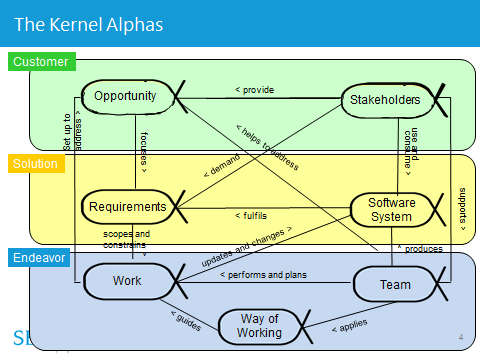
\includegraphics[scale=1, angle=360]{{img/essencekernel.png}}
  \centering
\end{figure}

\subsection{V-Modell}

\begin{figure}[H]
  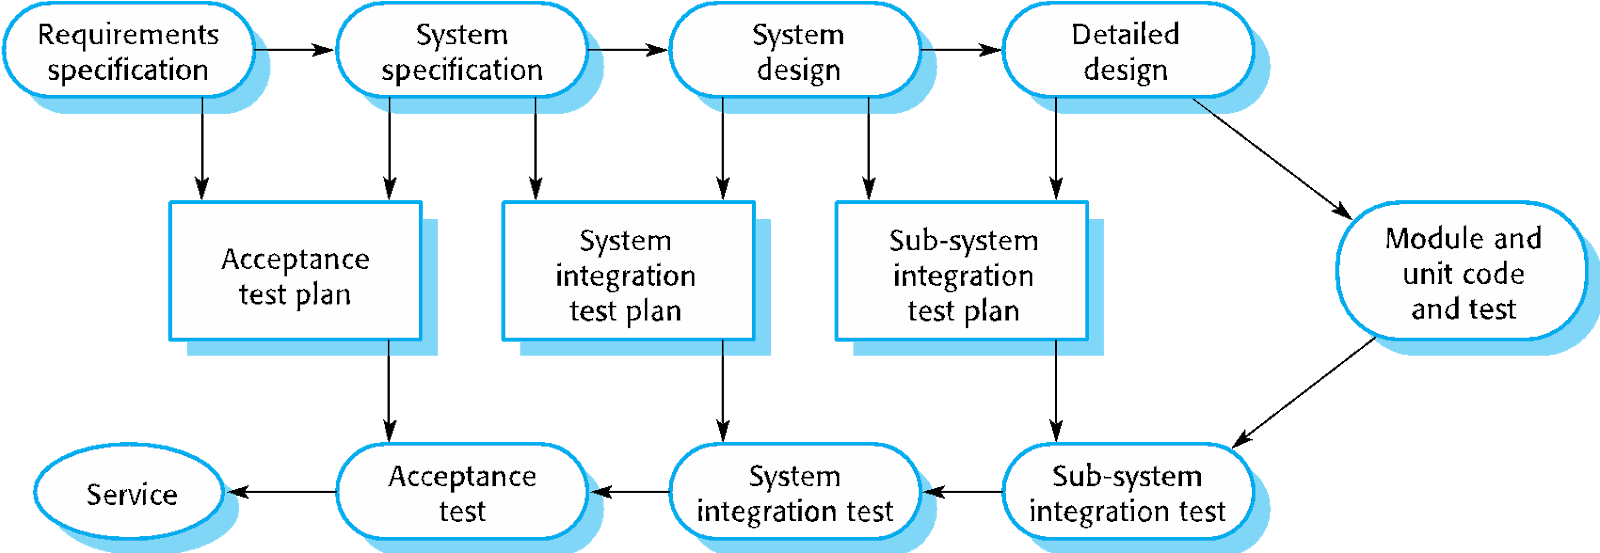
\includegraphics[scale=0.3, angle=360]{{img/vmodell.png}}
\end{figure}

\begin{enumerate}
  \item{Aus Anforderungen werden bereits einzelne Tests definiert}
  \item{Aus Anforderungen werden Systemspezifikationen festgelegt und weitere Tests geplant}
  \item{Nach der Spezifikation kommt das Design (Architektur); weitere Ausführung des Testplans}
  \item{Detailliertes designing der Module und Subsysteme}
  \item{Softwareentwickler schreiben die Module und machen die Tests}
  \item{Ist der Softwareentwickler fertig, wird auf der Subsystem Ebene begonnen zu integrieren und getestet mit dem Subsystem Plan}
  \item{Systemintegrationstest}
  \item{Abnahme des Kunden}
  \item{Ingebrauchnahme}
\end{enumerate}

$\rightarrow$ ist das Gegenteil von Agil!

\subsection{Sonstiges}
\subsubsection{Notizen zur ersten Übung}
Wichtig: Assoziativgesetz gilt nicht für Gleichkommazahlen $\rightarrow$ Rundungsfehler
Wenzel Algorithmus: 
\begin{enumerate}[label=(\alph*)]
  \item{Summe der positiven Zahlen angefangen mit der absolut kleinsten Zahl}
  \item{Summe der negativen Zahlen absteigend}
  \item{Summieren}
  \end{enumerate}

\subsubsection{Systemattribute}
Soziotechnische Systeme haben systemspezifische Attribute. \newline
Studierender besteht Prüfung nicht $\rightarrow$ bezieht sich nur auf den einzelnen Studenten.\newline
Fallen Studenten des ganzen Studengangs durch $\rightarrow$ Fehler im Studiengang.\newline
Menschen sind involviert $\rightarrow$ nicht deterministisch.\newline
\newline
\textbf{Funktionale Attribute}: Attribute die man sofort überprüfen kann
\newline
\textbf{Nicht Funktionale Attribute}: Interaktion zwischen Systemkomponenten (bspw. Performanz, Größe, Stabilität, usw…)

\subsubsection{Environmental Influences}
Technische Änderungen in Systemen können Auswirkungen auf die soziotechnischen Systeme haben. 
\newline
Solche Änderungen können Auswirkungen auf die Power Relationsships (Machtgefüge) in einem Unternehmen haben.


\chapter{Vorlesung 2 (05.12.2018)}
In der zweiten Vorlesung am 05.11.2018 wurde der zweite Teil des zweiten Foliensatzes \textbf{SWE P02 Introduction} und Teile des dritten Foliensatzes \textbf{SWE P03 Software Lifecycles} präsentiert. 

\subsection{Allgemeines}
In der Vorlesung am 05.12.2018 haben wir folgendes für uns mitgenommen:

\subsubsection{Risk Management}
Risk Identification $\rightarrow$ mögliche Quelle (Technologien $\rightarrow$ (Bsp BlockChain – Skaliert nicht)) \newline
Organisation $\rightarrow$ wie stabil ist die Organisation – muss oder wird umorganisiert werden ?! Schwierig bei laufendem Wechsel\newline
Requirements $\rightarrow$ Hauptgrund für die agile Arbeit \newline
\newline
Dabei muss man sich immer fragen $\rightarrow$ Wer ist betroffen? Wer geht die Risiken ein? Wenn wir die Risiken kennen und wissen wie man damit umgeht ist das die Grundlage dafür damit umzugehen.
\vspace{5mm}
\newline
\textbf{Ziel des Risikomanagement}
\begin{itemize}
  \item{Cannot guarantee lack of accidents}
  \item {reduces probability of accidents}
  \item {reduces cost per accident}
\end{itemize}


\subsection{Sonstiges}

\chapter{Vorlesung 3 (12.12.2018)}

\chapter{Vorlesung 4 (19.12.2018)}

\chapter{Hausübung}
Die Hausübung ist im Foliensatz \textbf{SWE P02 Motivation} auf der Folie 46 zu finden. 

\subsection{Requirements}
Die Requirements stellten sich wie folgt:
\begin{itemize}
  \item{3 inputs (a,b,c)}
  \item{a ungleich 0}
  \item{Plausibilität $(b^2 > 4ac)$}
  \item{x1 und x2 real}
  \item{Fehlerbehandlung}
  \item{Inputprüfung}
  \item{Korrekte Wurzel}
  \item{Reproduzierbarkeit}
  \item{maximal 500 msec pro Aufruf}
  \item{Incode-Doku}
  \item{Exceptions}
  \item{Testbarkeit}
  \item{Output Float (Liste)}
  \item{Genau 10 Stellen}
  \item{Auf die nummerische Genauigkeit achten}
\end{itemize}

\subsection{Implementierung}
Für die Implementierung wurde JAVA verwendet und folgende Klassen implementiert:
\begin{itemize}
  \item{Main}
  \item{QuadraticEquation}
  \item{AIsZeroException}
  \item{ImaginaryNumbersException}
  \item{QuadraticEquationTests}
\end{itemize}

\subsubsection{Main.java}
\begin{lstlisting}[basicstyle=\small]
import java.util.List;
import java.util.Scanner;

public class Main {


    public static void main(String[] args) {
        //Read Input from console
        Scanner s = new Scanner(System.in);
        System.out.println("Enter a value for a: ");
        double a = Double.parseDouble(s.nextLine());
        System.out.println("Enter a value for b: ");
        double b = Double.parseDouble(s.nextLine());
        System.out.println("Enter a value for c: ");
        double c = Double.parseDouble(s.nextLine());
        s.close();


        //Start the timer
        long start_time = System.nanoTime();

        //Create new QuadraticEquation Object
        QuadraticEquation q = new QuadraticEquation(a, b, c);
        try {
            List<Double> results = q.calc();
            // print results
            for(int i = 0; i < results.size(); i++) {
                System.out.format("%.10f %n", results.get(i));
            }
           //Thread.sleep(1000);
        } catch (ImaginaryNumbersException e) {
            e.printStackTrace();
        } catch (AIsZeroException e) {
            e.printStackTrace();
//        } catch (InterruptedException e) {
//            e.printStackTrace();
        } finally {
            long end_time = System.nanoTime();
            double difference = (end_time - start_time) / 1e6;
            System.out.println("Duration: (msec) ");
            if(difference < 500) {
                System.out.println(difference);
            } else {
                System.err.println(difference);
            }
        }

    }

}
\end{lstlisting}


\subsubsection{QuadraticEquation.java}
\begin{lstlisting}[basicstyle=\small]
  import java.util.LinkedList;
  import java.util.List;
  
  public class QuadraticEquation {
  
      //coefficients of quadratic equation ax^2 + bx + c = 0
      public double a;
      public double b;
      public double c;
  
      //Contains the results x1 and x2
      public List<Double> results;
  
  
      //Constructor
      public QuadraticEquation(double a, double b, double c) {
          this.a = a;
          this.b = b;
          this.c = c;
          results = new LinkedList<Double>();
      }
  
      //Calculation method for x1 and x2
      public List<Double> calc() throws ImaginaryNumbersException, AIsZeroException {
          if (a == 0) {
              throw new AIsZeroException();
          }
  
          double s1 = (-b + Math.sqrt(Math.pow(b, 2) - (4 * a * c))) / (2 * a);
          double s2 = (-b - Math.sqrt(Math.pow(b, 2) - (4 * a * c))) / (2 * a);
  
          if (Double.isNaN(s1) || Double.isNaN(s2)) {
              throw new ImaginaryNumbersException();
          } else {
              results.add(s1);
              results.add(s2);
          }
          return results;
      }
  }
\end{lstlisting}

\subsubsection{AIsZeroException.java}
\begin{lstlisting}
public class AIsZeroException extends Exception {
  public AIsZeroException() {
      super("The Quadratic Equation contains imaginary numbers!");
  }
}
\end{lstlisting}

\subsubsection{ImaginaryNumbersException.java}
\begin{lstlisting}
public class ImaginaryNumbersException extends Exception {
  public ImaginaryNumbersException() {
      super("The Quadratic Equation contains imaginary numbers!");
  }
}
\end{lstlisting}

\subsection{Unit Tests}
\subsubsection{QuadraticEquationTests.java}
\begin{lstlisting}[basicstyle=\small]
  import org.junit.jupiter.api.Test;
  import static org.junit.jupiter.api.Assertions.assertEquals;
  import static org.junit.jupiter.api.Assertions.assertThrows;
  
  import java.util.*;
  
  public class QuadraticEquationTests {
  
      // tested with
      // http://www.math.com/students/calculators/source/quadratic.htm
  
      @Test
      public void testCalculation() throws ImaginaryNumbersException, AIsZeroException {
          List<Double> results = new LinkedList<Double>();
  
          // first test a = 1, b = 5, c = 1
          results.add(-0.20871215252208009);
          results.add(-4.7912878474779195);
  
          QuadraticEquation q = new QuadraticEquation(1, 5, 1);
          assertEquals(results, q.calc());
          results.clear();
  
          // second test a = 1, b = 2, c = 3
          results.add(-0.45861873485089033);
          results.add(-6.541381265149109);
  
          QuadraticEquation q1 = new QuadraticEquation(1, 7, 3);
          assertEquals(results, q1.calc());
          results.clear();
  
      }
  
      @Test
      public void testException() {
          // third test
          QuadraticEquation q2 = new QuadraticEquation(1, 2, 3);
          assertThrows(ImaginaryNumbersException.class, () -> {
              q2.calc();
          });
  
          // fourth test
          QuadraticEquation q3 = new QuadraticEquation(0, 2, 3);
          assertThrows(AIsZeroException.class, () -> {
              q3.calc();
          });
      }
  
  }
\end{lstlisting}



% evtl. Abkürzungsverzeichnis:
\clearpage
\phantomsection
\addcontentsline{toc}{chapter}{Glossar}  % evtl. ersetzen durch \addcontentsline{toc}{chapter}{Abkürzungsverzeichnis}
\chapter*{Glossar} % evtl. ersetzen durch \chapter*{Abkürzungsverzeichnis}
\begin{acronym}
 \acro{ETW}{Energietechnik und Energiewirtschaft}
 \acro{SQL}{Structured Query Language}
 \acro{Bash}{Bourne-again shell}
\end{acronym}


\end{document}
